\chapter{Causality Tracking}
\label{cha:causality-tracking}
This chapter, addresses the use of Bluetooth sightings as a way to
acquire knowledge about the movement patterns of people. To do so, we
propose a new technique with adjustable accuracy capable of
representing the causality relation between visited places.

\section{Motivation and System Model}
\label{sec:ct-motivation}

The use of hash functions is often suggested as a data sanitation
technique in which a Bluetooth address is replaced by a digest from
which it is not be possible to recreate the original address. However,
this is also not suitable for large scale BT sensing. It would be
possible, even with minimal information about someone, to identify the
respective digest, and from that point onward, the digest would again
function as a unique identifier (\emph{pseudonym}).

There are examples, such as the Netflix
case~\cite{DBLP:journals/corr/abs-cs-0610105}, that show how
surprisingly easy it can be to personalize information that was being
proposed as anonymous (\emph{quasi-identifier}
~\cite{bettini2005protecting}) simply by adding some basic additional
knowledge to the system. This is also visible in other
domains~\cite{Ohm:2010tc}. Therefore, the systematic registration of
Bluetooth sightings done at multiple locations constitutes a privacy
threat in that it allows the creation of a surveillance system for
people.

The use of Bluetooth as an enabling technology to establish the flows
of people is not a new concept. There are several examples, be it
within a city~\cite{Oneill:2006vq}, outdoor
festival~\cite{versichele2012use} or shopping mall
~\cite{millonig2008shadowing}.

The model in which we base our work assumes the existence of a network
of heterogeneous and autonomous nodes that collaborate in the
tracking process of Bluetooth devices. These nodes may have access to
various types of information about the devices: their MAC address, the
timestamp of the sighting, the type of Bluetooth protocols supported
by the devices, among others.

Similarly to the Gate Counting scenario in Chapter
\ref{cha:gate-counting}, there is the possibility of using preexisting
resources (nodes). As a consequence, our model does not impose
restrictions on the type of information registered by the
scanners. The nodes will continue to perform the same functions they
did before. Our concern is to the information that
might be exchanged by the nodes in the context of collective tracking,
 and to the privacy risks that might ensue such as the ability
to accurately follow the movement of a device and therefore of its
respective owner.

In their everyday life and depending on their specific needs, people
visit several different places. For instance, a person $P_1$ wants to
buy a new laptop. To do so, she visits store $S_1$ which does not have
the model she wants. She then visits store $S_2$ which is out of
stock and afterwards store $S_3$ where the price is a little
steep. She ends up buying the laptop in store $S_4$. To represent this
behavior we introduce the concept of \emph{mobility traces}. A
mobility trace is simply the representation of the places visited in the
order by which they were visited. In this specific case, the mobility
trace of $P_1$ is $MT_{P_1}=\{S_1,S_2,S_3,S_4\}$. Our mechanism,
\emph{Precedence Filters}, allows the recording of information
relative to the individual traces of people, in a manner compatible
with plausible deniability. That information can later be
processed/mined to obtain more accurate data about the habits of the
aggregate of all individuals. For instance, in this example, the order
in which the stores were visited might be an indicator of their
reputation/popularity.

A common strategy that seeks to strengthen privacy is the restriction
of captured data to just the essential. In our specific case, the goal
is the detection of movement patterns between nodes. As such, the
ability to detect the same device on different nodes is fundamental. To
minimize the amount of information collected, we can ignore
information such as the duration of the sightings, the timestamp in which
they occurred, the device name, supported Bluetooth protocols,
among others. We just need the device's MAC address.

Whenever a device is sensed, the sighting node records that event
locally. This information is then used in the computation of device
transitions between the system's multiple nodes. The place where that
computation occurs depends on the system's architecture. Our mechanism
can be deployed in either centralized or decentralized
architectures. In a centralized system configuration, the computation
has to be done in the server since only it has enough information to
do so. Each node only shares its local information with the server. On
the other hand, with a decentralized architecture, nodes can do the
processing locally. The local information each node possesses is
shared with the other nodes, thus allowing all the nodes to have
access to the data. Both models have advantages and
disadvantages. For instance, the centralized approach is not fault
tolerant, if the server crashes the tracking system stops
working. This does not happen in the decentralized approach given that
the same information is stored in multiple nodes (redundancy). The
system can keep on working even if some of the nodes fail. Compared to
the centralized version, the decentralized model also has greater
availability as a result of the information redundancy. However, as a
consequence of the exchange of information between all the nodes, the
decentralized scenario has a bigger burden on the network when
compared to the centralized one.


In order to achieve the goal we set ourselves, and taking into account
the constrains presented by our model, our solution is based upon the
following set of assumptions:
\begin{itemize}
\item Even though we cannot make assumptions about how each individual
  node will handle the observed Bluetooth addresses, our solution
  should never require the Bluetooth address or any other information
  that could uniquely identify individuals to ever leave the sensing
  node.
\item No system element should, at any given time, have all the
  information necessary to accurately determine the path of a single
  individual.
\item The aggregate result that a node can create about the set of all
  visiting devices should be accurate enough to be useful in human
  mobility observation scenarios, e.g. most common paths, similarity
  level between places.
\item There are no communication failures in the system and the
  exchange of information between any two nodes is faster than the
  time it takes for a person to move between them. This ensures that
  the order in which the sightings are recorded is correct, i.e., when
  a person goes from node $A$ to node $B$, node $B$ must already
  have the information that she was in $A$.
\end{itemize}

\subsection{Objectives}
\label{sec:ct-objectives}
In this chapter, we discuss the use of Bluetooth sightings, captured
by a group of cooperative scanners, with the purpose of obtaining
information about the movement patterns of users. All without
compromising their privacy. Particularly, we wish to explore the
application of stochastic summarizing techniques as a privacy preserving
approach to Bluetooth Tracking.

The technique presented in this chapter, Precedence Filters (PFs), gives
each Bluetooth scanner the ability to obtain probabilistic information
about the provenance of the detected visitors. This information
concerns the nodes that were visited just prior to the current
scanner. Its accuracy can be adjusted to an uncertainty level
compatible with plausible deniability. This means that it must be
reasonable to believe an individual who denies being in a given place
even if the stochastic technique points otherwise.
 % Even so, the information about the aggregate of
% all visitors must have enough accuracy to be relevant in the study of
% the group's movement patterns.
However, when considering the aggregate view of all the visits, the
algorithm is able to provide enough accuracy to be a relevant source
of data for Human mobility studies.

\section{Precedence Filters}
\label{sec:precedence-filters}
By applying some of the previously mentioned (Subsection
\ref{sec:vector_clocks}) general constructs of distributed systems to
the mobility sensing scenario, Bluetooth scanners can be treated as
processes and device sightings as state transition events. Precedence
Filters are based upon this idea and provide accurate mobility
information, at a macroscopic level, without neglecting individual
privacy.  Precedence Filters can be seen as a vector clock
\cite{Fidge,Mattern} implementation, whose difference is the use of
Counting Bloom Filters~\cite{Fan98summarycache:,Mitzenmacher:2002:CBF:581876.581878} (one for each node in the system) by the PFs
instead of integers (one per process) used by vector clocks.

In the decentralized model each Bluetooth node has its own PF and the
nodes communicate with each other upon sighting events in order to
keep their filters updated. On the other hand, in the centralized
approach, each node possesses a simple CBF, whose updates can only be
made through communication with the centralized server.  The
centralized server maintains an up to date copy of each node's CBF,
i.e., a Precedence Filter.

\begin{figure}
  \centering
  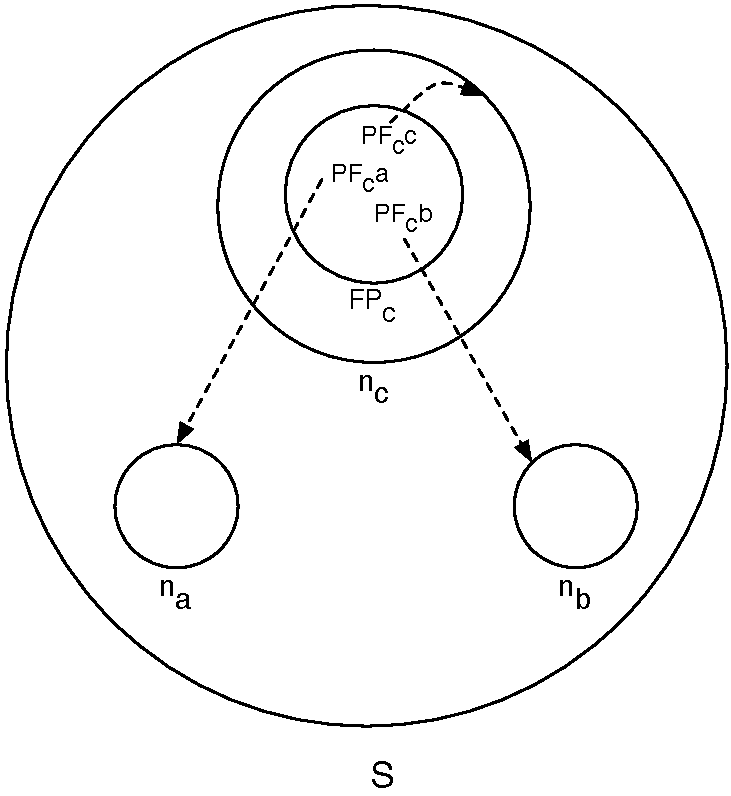
\includegraphics[width=0.60\textwidth]{images/precedence_filters.pdf}
  \caption{Diagram of relevant entities and data structures}
  \label{fig:precedence_filters}
\end{figure}

Our work is based in the decentralized approach. Both our
implementation and the tests we ran are based upon it. So,
from now on, we will be referring to the decentralized version only,
although it is not hard to draw conclusions that apply to the
centralized scenario as well.
With that in mind, Precedence Filters work as follows: supposing we
have a set of Bluetooth scanners (nodes) $S$, each node $n \in S$ has
a Precedence Filter $PF_n$. That PF is in turn composed of a map of
\emph{Counting Bloom Filters}, one for each node $z \in S$. We use
notation $PF_n^z$ to refer to the CBF for scanner $z$ belonging to
$PF_n$, as depicted in Figure ~\ref{fig:precedence_filters}.

All CBFs are initially set to 0, use the same set of hash functions
$K$ and have the same size $M = m * k$ ($k$ is calculated with
equation \ref{eq:optimal_hash_number} and $m$ is calculated with
equation \ref{eq:optimal_slice_size}). This ensures that the same
device is correctly identified across the several nodes (upon
detection it will be mapped to the same indices). Precedence Filters
can also be seen as a matrix where the number of rows is equal to the
number of nodes in the system and the number of columns is equal to $M$.

Each time a node $n$ detects a device $d$, its Precedence Filter
$PF_n$ is updated according to the following set of rules:
\begin{enumerate}
\item Using the set of hash functions $K$, the node $n$ calculates the
  set of indices $I_d$. $I_d$ consists on the output from the $K$ hash
  functions regarding device $d$, $I_d=\bigcup_{f \in K} f(d)$.
\item Node $n$ sends the set of indices $I_d$ to all other nodes
  in $S$.
\item Each one of the $z$ nodes belonging to $Z$ ($Z = S \backslash
  \{n\}$) replies with a set of tuples $R_z^{I_d}$. $R_z$ contains
  the previously required $I_d$ along with the set of values that each
  of the CBFs belonging to $FP_z$ had stored in those indices,
    $R_z^{I_d}= \{(i,PF_z^z[i]) \mid \forall i \in I_d \}$.
\item Upon the reception of the replies from the other nodes, $n$
  updates its own indices $I_d$ on the CBFs relative to the other
  nodes with the maximum value received, $PF_n^z[i] = \max(R_z^{I_d}[i]), \forall
  z \in Z, \forall i \in I_d$, where $R_z^{I_d}[i] = v \rightarrow (i,v) \in R_z^{I_d}$.
\item Lastly, $n$ updates the indices $I_d$ on its own CBF
  ($PF_n^n$). For each index $i \in I_d, PF_n^n[i] = \max(PF_n^s[i])+1,
  \forall s \in S$. By adding 1 to the maximum value stored in the
  other nodes, the current node ``dominates'' them in the operation
  that returns the causality between the visited places. In other
  words, this is the key to obtaining the order in which the places were
  visited.
\end{enumerate}

This set of rules allows the precedence filters to record information
about the precedence of the locals visited by a device. Given a set of
indices $I_d$ for device $d$ and any pair of scanners $x$ and $y$, we
say that the sighting of $d$ in $x$ precedes the one in $y$, $x
\leadsto y$ if:

\begin{center}
\begin{math}
	x\leadsto y \Longleftrightarrow PF_{x}[I_d] < PF_{y}[I_d]
\end{math}
\end{center}
Where $PF_x[I_d] < PF_y[I_d]$ stands for:
\begin{center}
  \begin{math}
    \forall i \in I_d : PF_x^x[i] < PF_y^y[i]
  \end{math}

\end{center}
It is easy to see the similarities with the vector clock description
from Subsection \ref{sec:vector_clocks}.

Mobility traces, used in our model to describe the behavior of
individuals, characterize a total order between the places
visited. This means that it is always possible to establish an order
between any two places in the mobility trace. However, being based upon the
happens-before relation~\cite{Lamport:1978}, Precedence Filters can
only represent partial orders. In this particular case, for each of
the nodes/locations, they can only ``remember'' the last time each
device was sighted in a given place. For instance, given the mobility trace
$MT_{P}=\{S_1,S_2,S_1,S_3,S_2,S_4,S_1\}$ where scanners $S_1$ and $S_2$
are visited more than once, in the best case scenario PFs can obtain
$CT_{P}=\{S_3,S_2,S_4,S_1\}$, which we will refer as a \emph{causality
 trace}. This is a consequence of the irreflexivity and antisymmetry
properties from the happens-before relation. However, we can look at
this as a feature of Precedence Filters, a sort of automatic data
degradation. It ensures that the length of the record of sightings for any given
device has an upper bound equal to the number of Bluetooth scanners in
the tracking system.

The level of privacy offered by Precedence Filters can be further
customized by adjusting the CBFs' false positive ratio (Equation
\ref{eq:false_positive}). The higher the ratio, the greater the
inaccuracy of the PFs. The occurrence of false positives in the CBFs
results in the appearance of \emph{fictitious transitions}, i.e., the
causal trace obtained from querying the filters, contains transitions
which are non-existent in the original trace.

Both these properties are what allow individual users to plausibly deny the
fidelity of the data extracted from the Precedence Filters.

\section{Metrics and Data Sets}
\label{sec:metrics-data-sets}

To assess the performance of Precedence Filters we compared the set of
transitions obtained from querying the Precedence Filters with the set
of transitions obtained from the causality traces, which were
themselves obtained from mobility traces.  For instance, given the
mobility trace $MT_P=\{S_1,S_2,S_2,S_1,S_3\}$, we calculate its
causality trace according to the happens-before relation (that only
contains last sighting in each place), $CT_P=\{S_2,S_1,S_3\}$. Then we
extract the set of transitions, denoted as $\mathcal{T}$, from that causality trace,
$\mathcal{T}(CT_p)=\{(S_2,S_1),(S_2,S_3),(S_1,S_3)\}$. Each transition is a two location
tuple where the first location causally precedes the second. In our
scenario, that means the device was seen in the first location before
being sighted at the second location. This set of transitions is then
finally compared to a similar set of transitions obtained from the PFs.


\subsubsection{Metrics}

The performance of Precedence Filters is measured according to two
different metrics.

The \emph{individual} metric which measures the
false probability of statements like the following - ``
individual $X$ visited location $S_1$ before visiting location
$S_2$''. For each user $u$, this is done by calculating the cardinality of the mutually
exclusive set between the transitions belonging to the causality trace
($\mathcal{T}(CT_u)$) and the transitions extracted from the Precedence Filter
($\mathcal{T}(PF_u)$), according to Equation \ref{eq:complex_individual_metric}.
 \begin{equation}
   \label{eq:complex_individual_metric}
   \frac{\# ( (\mathcal{T}(CT_u) \bigcup \mathcal{T}(PF_u) )
       \setminus (\mathcal{T}(CT_u) \bigcap \mathcal{T}(PF_u) ) )}
     {\#(\mathcal{T}(PF_u))}
 \end{equation}
 Figure \ref{fig:venn_diagram_complex}, which is the Venn diagram
 representation of Equation \ref{eq:complex_individual_metric}, shows
 that the individual metric calculates the relative amount of
 incorrect information (information that is on the CTs and not on the
 PFs and \textit{vice-versa}) returned by the Precedence
 Filters. However, given the assumption that the exchange of
 information between nodes is faster than people, our system never
 forgets information, i.e., $\mathcal{T}(CT) \subseteq
 \mathcal{T}(PF)$. Therefore, Equation
 \ref{eq:complex_individual_metric} can be simplified, resulting in
 Equation \ref{eq:simple_individual_metric} as depicted in Figure
 \ref{fig:venn_diagram_simple}.

\begin{figure}
  \centering
  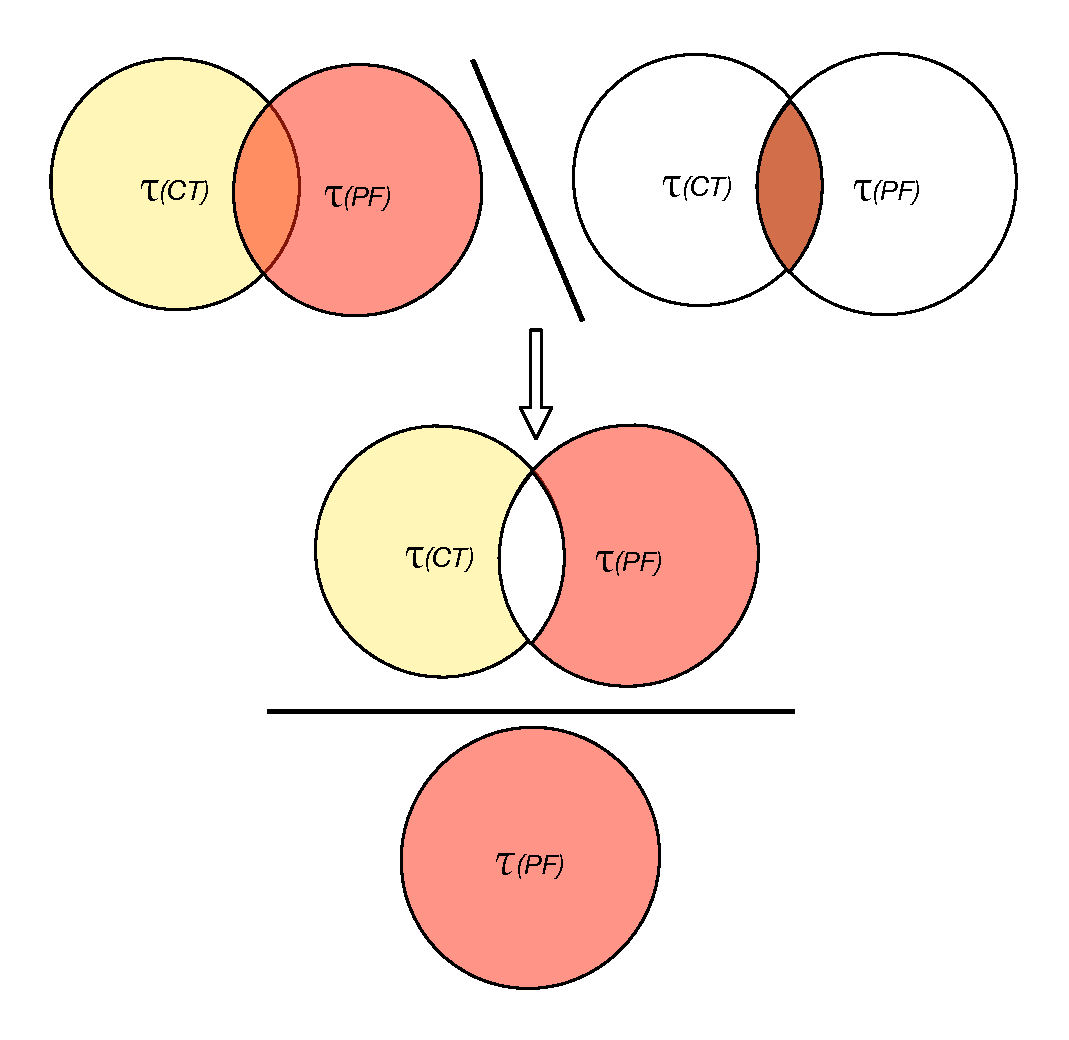
\includegraphics[width=0.50\textwidth]{images/venn_diagrams_complex.pdf}
  \caption{Venn diagram representation of Equation \ref{eq:complex_individual_metric}}
  \label{fig:venn_diagram_complex}
\end{figure}

 \begin{equation}
   \label{eq:simple_individual_metric}
   \frac{\# ( \mathcal{T}(PF_u) \setminus \mathcal{T}(CT_u) )}
     {\#(\mathcal{T}(PF_u))}
 \end{equation}

\begin{figure}
  \centering
  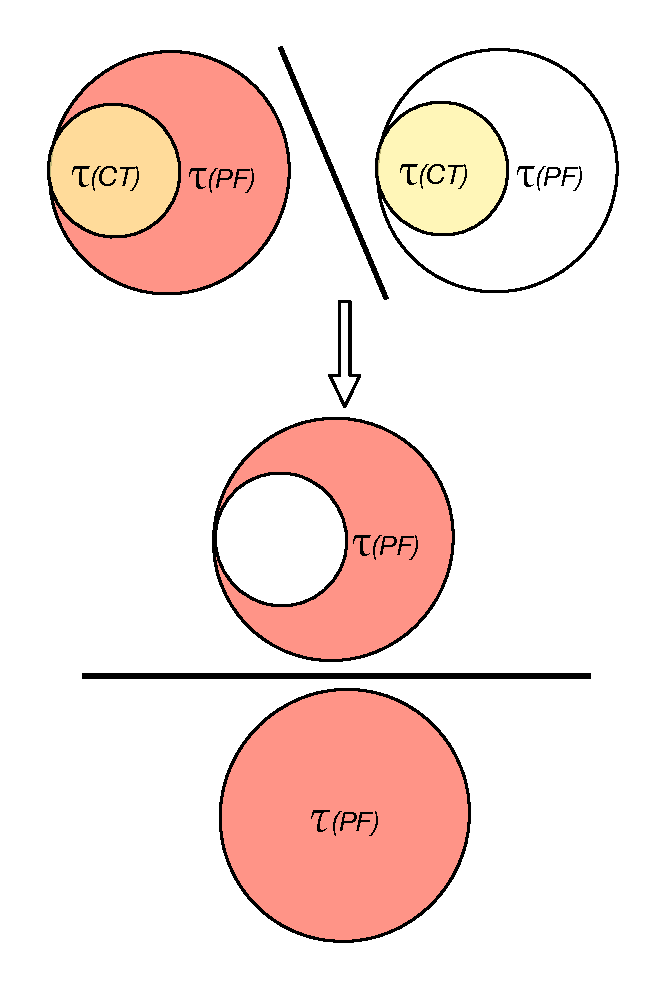
\includegraphics[width=0.35\textwidth]{images/venn_diagrams_simple.pdf}
  \caption{Venn diagram representation of Equation \ref{eq:simple_individual_metric}}
  \label{fig:venn_diagram_simple}
\end{figure}

 The \emph{global} metric quantifies the inaccuracy of information
 regarding the relative weight of specific transitions. This enables
 us to establish the relative importance of each type of transition,
 i.e., to know the inherent error in statements like - ``2\% of the
 transitions are from Restaurant Y to Cafe Z''.  Assuming that, $U$
 represents the universe of all users, $\mathcal{A}_{PF} = \biguplus_{u \in
 U} \mathcal{T}(PF_u)$ and $\mathcal{A}_{CT} = \biguplus_{u \in
 U} \mathcal{T}(CT_u)$ are respectively the multiset union of all transitions
in the Precedence Filters and in the Causality Traces and that
$\mathcal{A}[t]$ is multiset composed only of the $t$ transitions in
$\mathcal{A}$, the global metric for each transition $t \in
\mathcal{A}$ is calculated according to equation
\ref{eq:global_metric}. For each transition, we calculate the
absolute difference between its relative weight in the Precedence Filter and
its relative weight in the actual Causality Traces. Then we divide that number
by its weight on the Precedence Filters. This gives us the
relative error of the relative weight of the transition.

\begin{equation}
  \label{eq:global_metric}
   \frac {\left| \frac{ \# \mathcal{A}_{PF}[t]}{\#\mathcal{A}_{PF}} -
    \frac{\#\mathcal{A}_{CT}[t]} {\# \mathcal{A}_{CT} }\right|}
{\#\mathcal{A}_{PF}[t]}
 \end{equation}

% The \emph{global} metric quantifies the relative weight of
%  one transition (e.g. $(S_1,S_3)$) against the total number of
%  transitions recorded. For each type of transition, its total number
%  of occurrences is divided by the sum of total number of occurrences
%  of all transitions. By doing so we are able to establish the relative
%  importance of each type of transition, i.e. to make affirmations like
%  - ``2\% of the transitions are from Restaurant Y to Cafe X''.
%  \todo{Arranjar Fórmula para métrica global}

\subsubsection{Real Data set}

To evaluate the PFs' performance we used a real data set with
information about Bluetooth sightings by static nodes. This data set
was taken from Leguay et al.'s work~\cite{leguay2006opportunistic}. To
collect this information, the authors handed out a set of Bluetooth
enabled devices called \emph{iMotes} to a group of users who carried
them in their day-to-day. Additionally, the authors installed
Bluetooth scanners in several places with the purpose of registering the
sightings of \emph{iMotes}. The dataset contains 18 static nodes and
9244 distinct device IDs, 6439 of which have been sighted only once
and were therefore removed. This leaves us with 2805 devices, whose
average mobility trace size is approximately 4 and maximum size is
11. Figure \ref{fig:dev_sig_real} shows the distribution of total and
distinct sightings for all scanners. As expected, not all places have
the same popularity, some are more visited than others, thus the
bigger number of Bluetooth sightings.

\begin{figure}[htb]
\subfigure[Real data set]{
\label{fig:dev_sig_real} 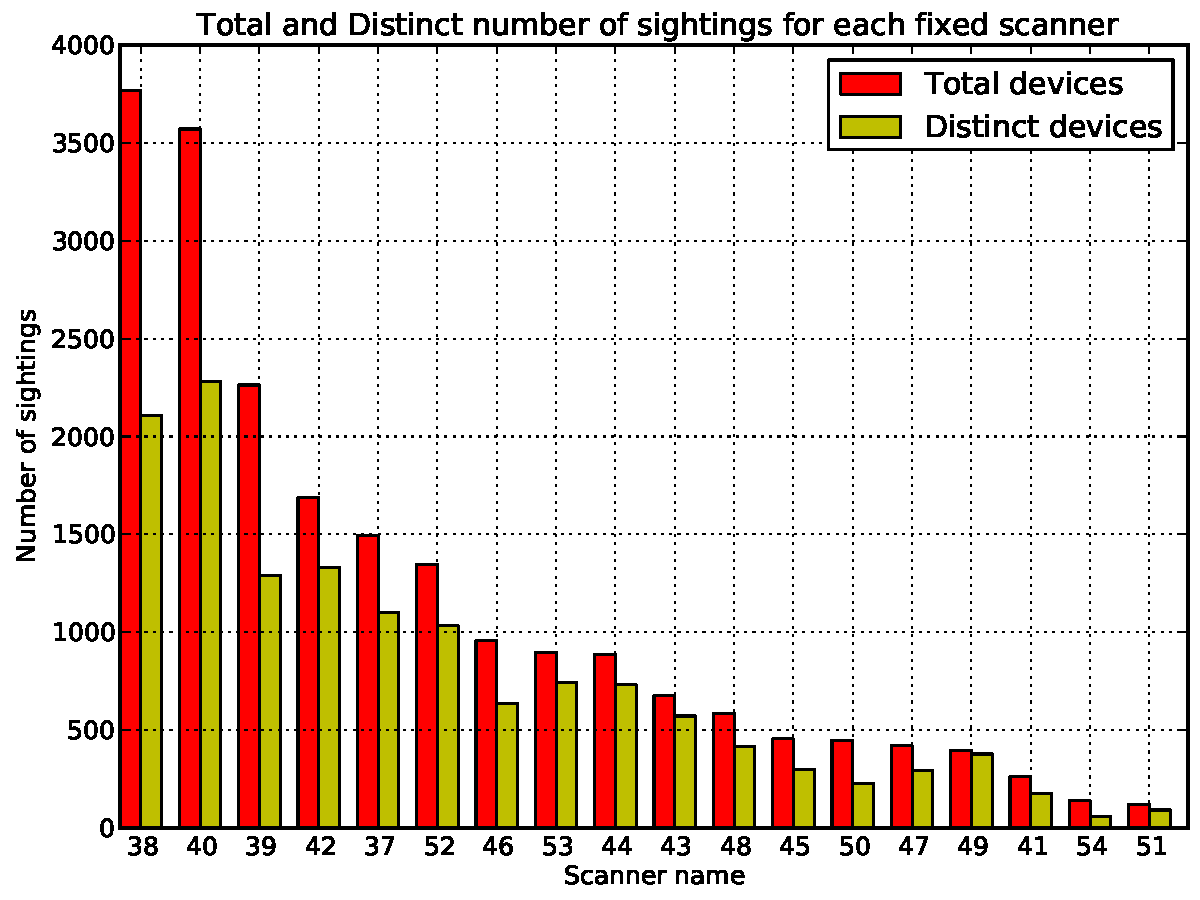
\includegraphics[scale=0.33]{images/rTotalDistinctSightings.pdf}
} \subfigure[Synthetic data set]{
 \label{fig:dev_sig_synthetic}  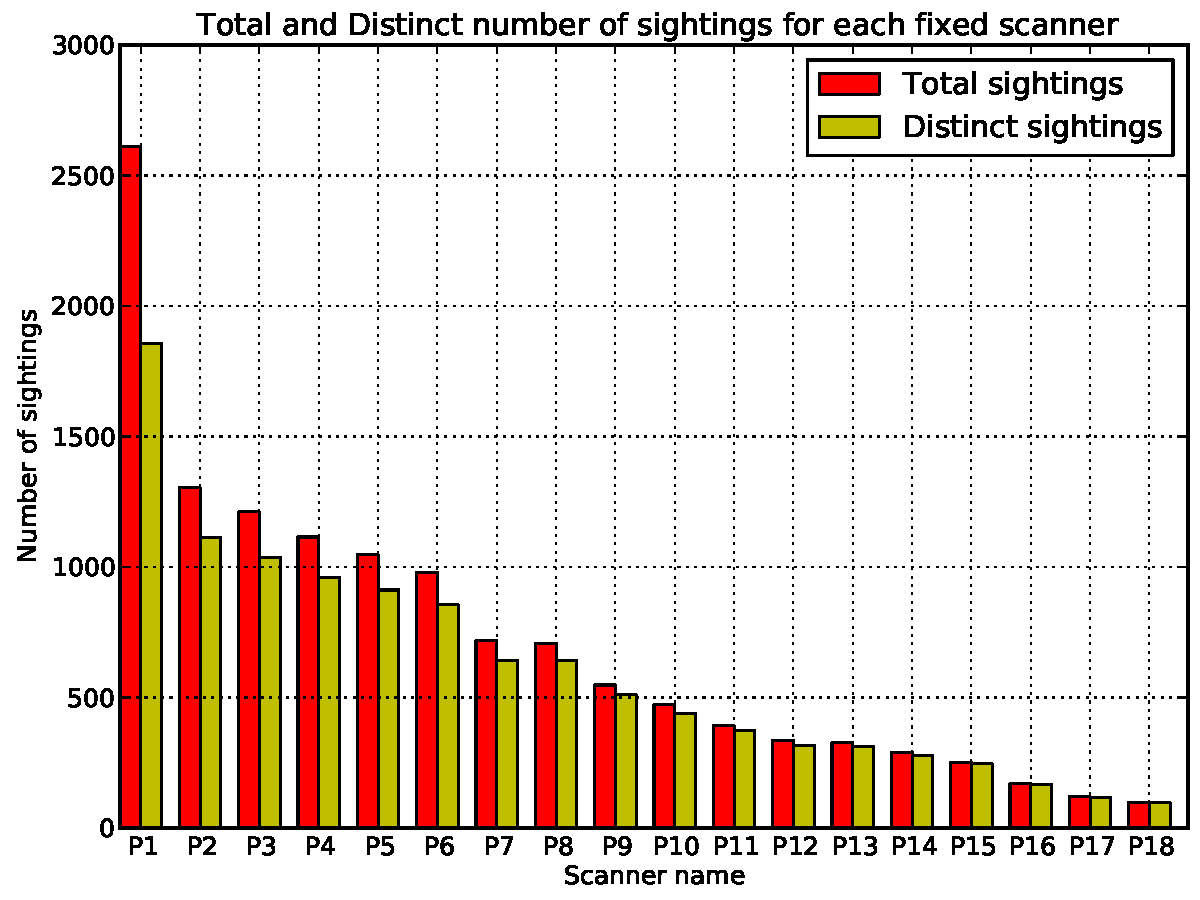
\includegraphics[scale=0.33]{images/sTotalDistinctSightings.pdf}
}
\caption{Number of total and distinct device sightings across the scanners}
\label{fig:deviceSightings}
\end{figure}

\subsubsection{Synthetic Data Set}
\label{sec:simulator}

Still in the context of evaluating the PF's performance, we built a
synthetic trace generator. Our motivation came from the need to
simulate scenarios with arbitrary number of locations and users.

In a first approach, we tried fitting the statistic distribution of
the real data set using a negative exponential distribution. This
would have allowed us to choose an arbitrary number of sensors, users
and trace length. However, after evaluation with Pearson's Chi-Square
test, it turned out to be a bad fitting. This might be solvable by
switching to a more complex distribution function. Instead we chose to
work with the empiric distribution.
On this second approach, it was decided to use the same number of sensors
as the real data set, i.e. 18. This allowed us to simulate the
popularity of each sensor/place using the number of sightings from the
real data set as weights. The larger the number of sightings at a
sensor, the bigger its weight is, and the more likely it is to be
chosen. Each node is defined by two parameters, unique sightings and
total sightings. We only made use of the latter. The use of
\emph{replication}\footnote{In statistics, replication is the
  repetition of an experiment or observation in the same or similar
  conditions.} enabled us to create  a simpler and less error prone
simulator, capable of producing as many users as we want, as well as
mobility traces with arbitrary length.  The downside of not using the
unique number of sightings is that we are assuming that even though
places have different weights, they are the same for everyone,
i.e. everyone has the same probability of choosing a given place,
everyone is an ``average'' person.

Figure \ref{fig:dev_sig_synthetic} shows the synthetic distribution
obtained using the approach mentioned above.  As expected the results
are very similar but not a perfect match. There is a
correlation between the number of total and unique sightings which
stems from the use of the ``average'' person model. Also, the curve from the
synthetic data set is smoother, it does not suffer from the
``noise'' inherent to raw real data.

\section{Evaluation}
\label{sec:ct-evaluation}

Using the metrics and data sets previously mentioned, we tested the
Precedence Filter's inaccuracy across several scenarios, varying both
the number of devices and the length of the mobility traces.
Furthermore, each of the scenarios was tested with multiple different
settings for the Counting Bloom Filter's maximum false positive
probability (see Equation \ref{eq:false_positive}).
A good performance is reflected through high inaccuracy values for
individual information together with low values for global inaccuracy.

As can be seen in Figures \ref{fig:perf_results_real_sim},
\ref{fig:perf_results_sim_device_number},
\ref{fig:perf_results_sim_trace_size} and
\ref{fig:perf_results_sim_devices_traces}, by increasing the false
positive probability of CBFs, inaccuracy increases as well.
Inaccuracy is manifested via the occurrence of fake (visible on PFs
only) transitions, i.e., \emph{fictitious transitions}. As the false
probability increases, so does the percentage of fake transitions.
This is easily explainable. In Bloom Filters, false positives denote
elements wrongfully considered as belonging to the set.  Given that in
PFs Bloom Filters are used to record device sightings, the occurrence
of false positives generates fake device sightings, which in turn give
origin to fictitious transitions.

As previously explained, both data sets use 18 scanning nodes, what
differs is the number of devices and the length of the mobility
traces. To describe the parameters of each scenario, the following
notation is used in the captions: Synthetic/Real-[\emph{number of
  devices}]-[\emph{maximum trace length}]-[\emph{average trace
  length}].

\begin{figure}[htb]
\centering
\subfigure[Synthetic-2805-11-4]{
\label{fig:ss_2805_11_4}  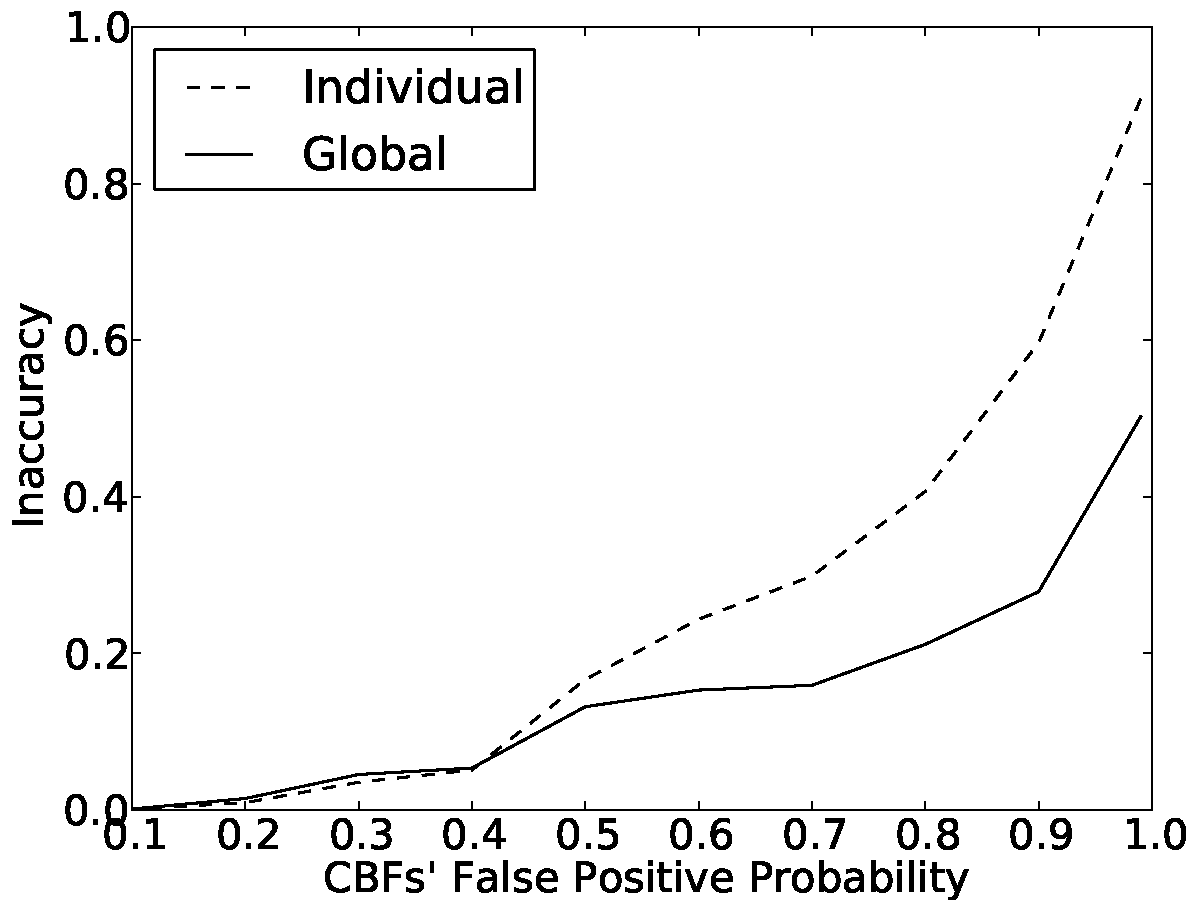
\includegraphics[width=0.33\linewidth]{images/s18x2805x11x4.pdf}
}\hspace*{-0.7em}
\subfigure[Real-2805-11-4]{
  \label{fig:r_2805_11_4} 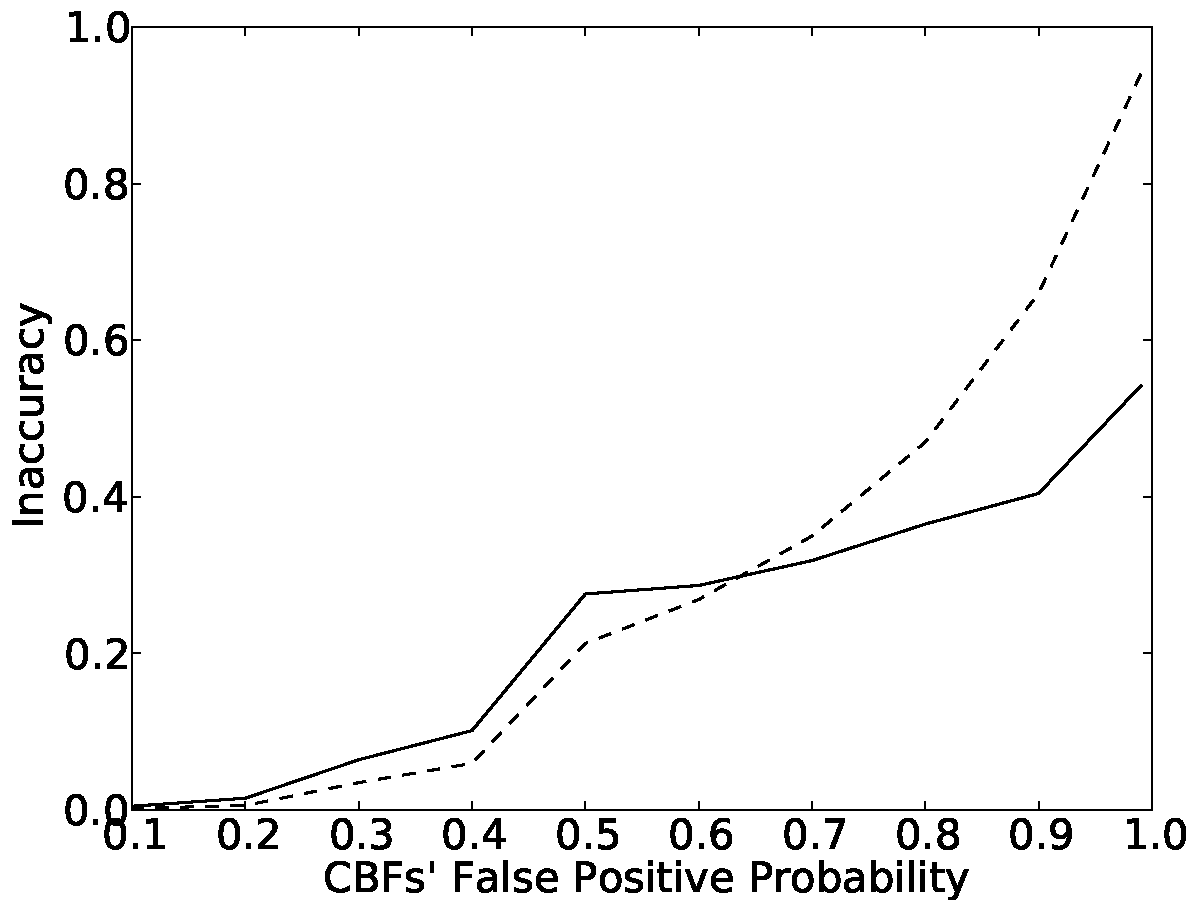
\includegraphics[width=0.33\linewidth]{images/r18x2805x11x4.pdf}
}
\caption{Comparison between real and synthetic data set, with same parameters}
\label{fig:perf_results_real_sim}
\end{figure}


Figure \ref{fig:perf_results_real_sim} shows the comparison between a
synthetic data set and the real data set. This synthetic data set will
serve as the baseline for all tests because it simulates both the
number of devices and trace length found in the real data set.  Our
technique performs better with data from the synthetic data set
(Figure~\ref{fig:ss_2805_11_4}) than it does with data from the real
one (Figure~\ref{fig:r_2805_11_4}).  This is a consequence of the
average person simplification we did for the synthetic data
sets. Figure \ref{fig:deviceSightings} shows that while the number of
total sightings is approximately equal in both data sets, the number
of unique sightings is usually bigger in synthetic data set.  This
means that the real data set has a greater number of repeated
sightings by user, which in turn means that the average length of the
causality traces is smaller, i.e., even if both data sets have the same
number of users and similar sized mobility traces, the causality
traces in the real data set are smaller, explaining the worse
performance of our technique.

For both
these data sets, there is a point where the individual accuracy is
greater than the global one, however, when the individual inaccuracy
is approximately $50\%$, the global inaccuracy is higher than what is
desirable. This is a result of the low number of individuals and small
mobility trace sizes of both data sets, as supported by Figures
\ref{fig:perf_results_sim_device_number},
\ref{fig:perf_results_sim_trace_size} and
\ref{fig:perf_results_sim_devices_traces}.

\begin{figure}[htb]
\subfigure[Synthetic-2805-11-4]{
\label{fig:s_2805_11_4_1}  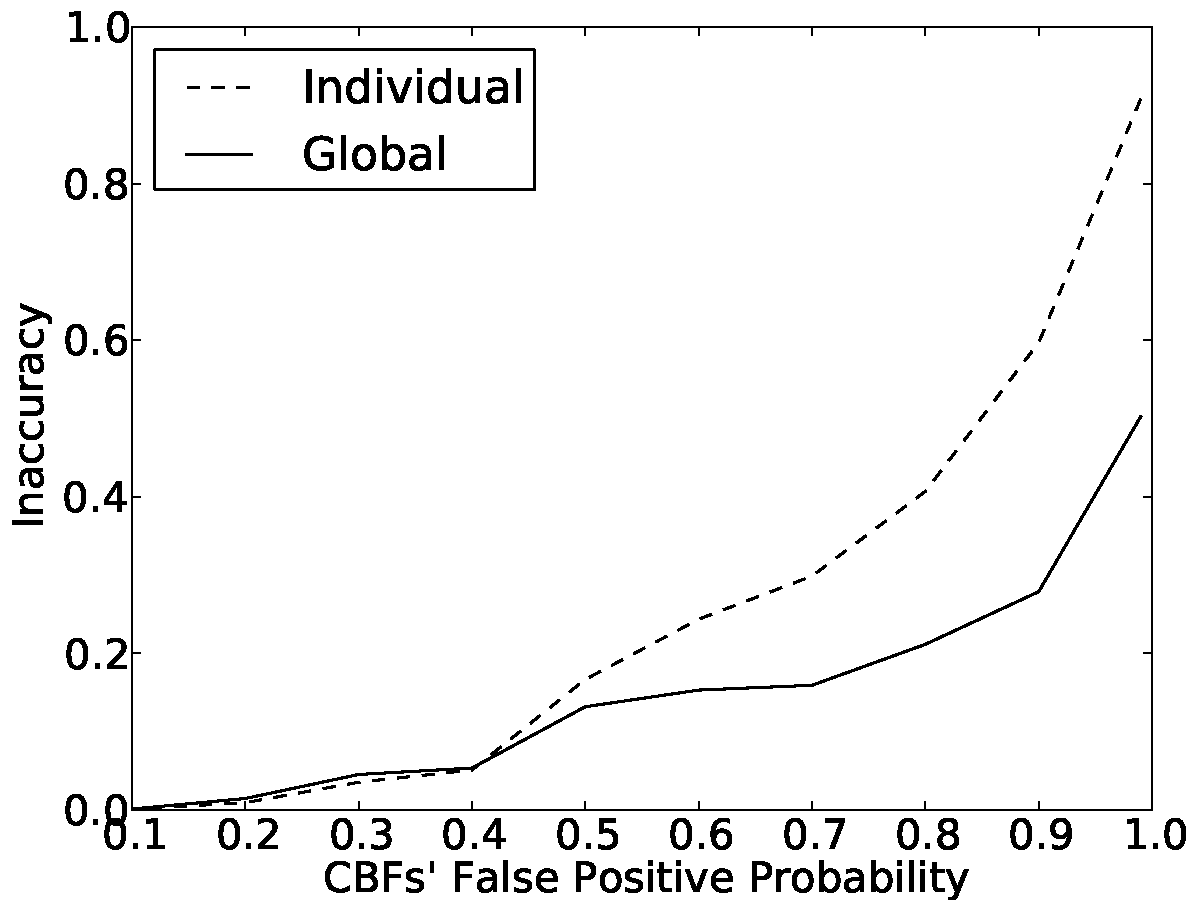
\includegraphics[width=0.33\linewidth]{images/s18x2805x11x4.pdf}
}\hspace*{-0.7em}
\subfigure[Synthetic-10000-11-4]{
 \label{fig:_10000_11_4}  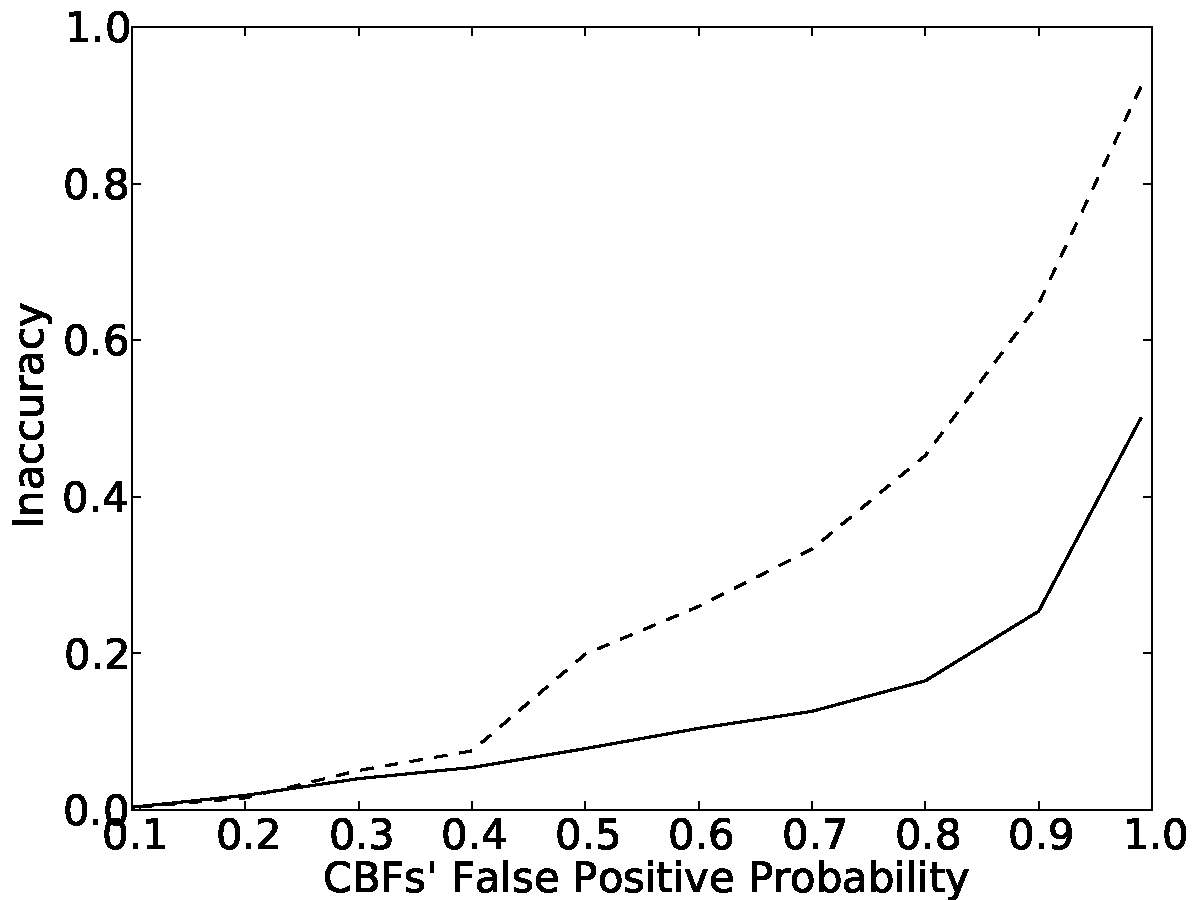
\includegraphics[width=0.33\linewidth]{images/s18x10000x11x4.pdf}
}\hspace*{-0.7em}
\subfigure[Synthetic-100000-11-4]{
\label{fig:s_100000_11_4}  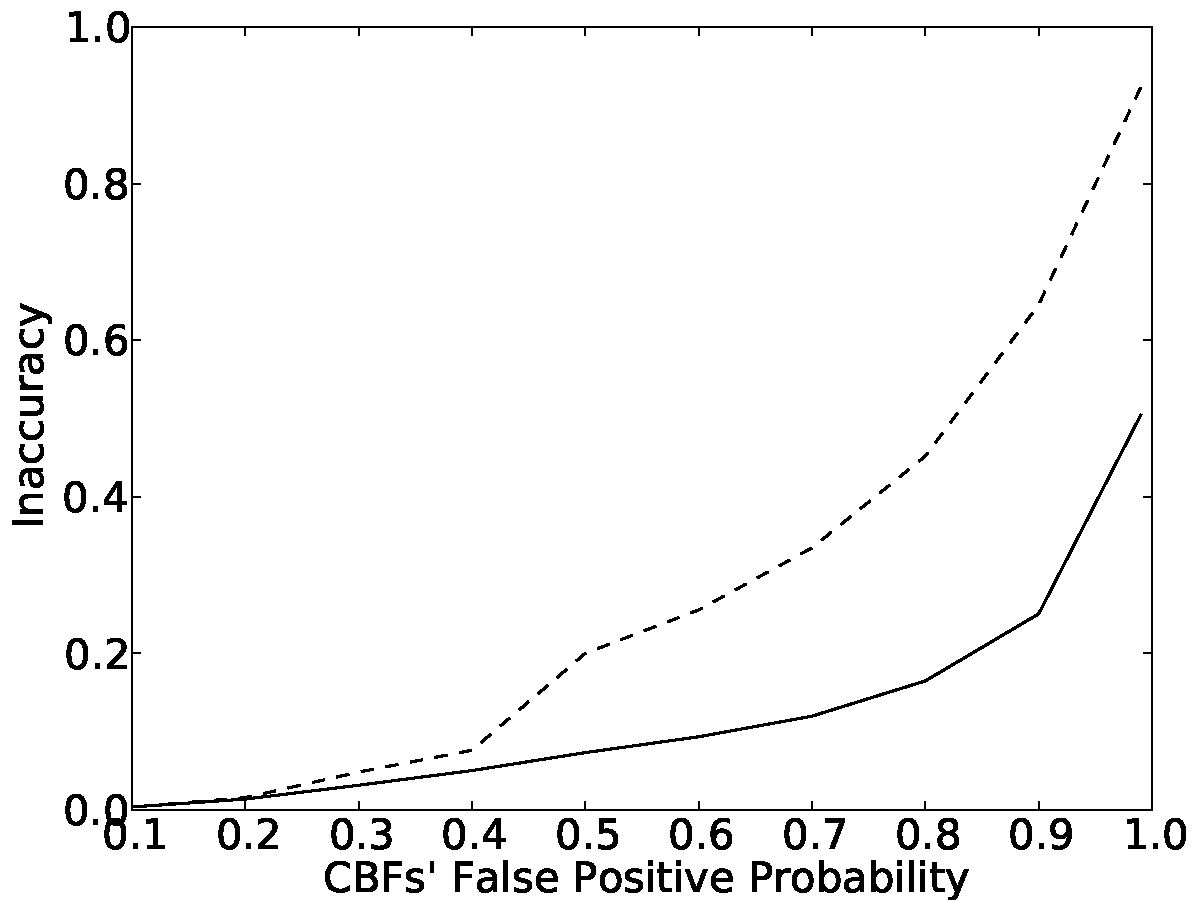
\includegraphics[width=0.33\linewidth]{images/s18x100000x11x4.pdf}
}
\caption{Synthetic data sets with increasing number of devices}
\label{fig:perf_results_sim_device_number}
\end{figure}
Maintaining the length of mobility traces constant, Figure \ref{fig:perf_results_sim_device_number} shows that Precedence
Filter's global inaccuracy drops by increasing the number of devices
to 10 000, and then again, although little, by increasing that number
to 100 000. In both scenarios, for a false positive probability of
$0.8$, PFs provide global inaccuracy below $20\%$ while ensuring that
in average, $50\%$ of the information about any given individual is
incorrect.


\begin{figure}[htb]
\subfigure[Synthetic-2805-11-4]{
\label{fig:s_2805_11_4}  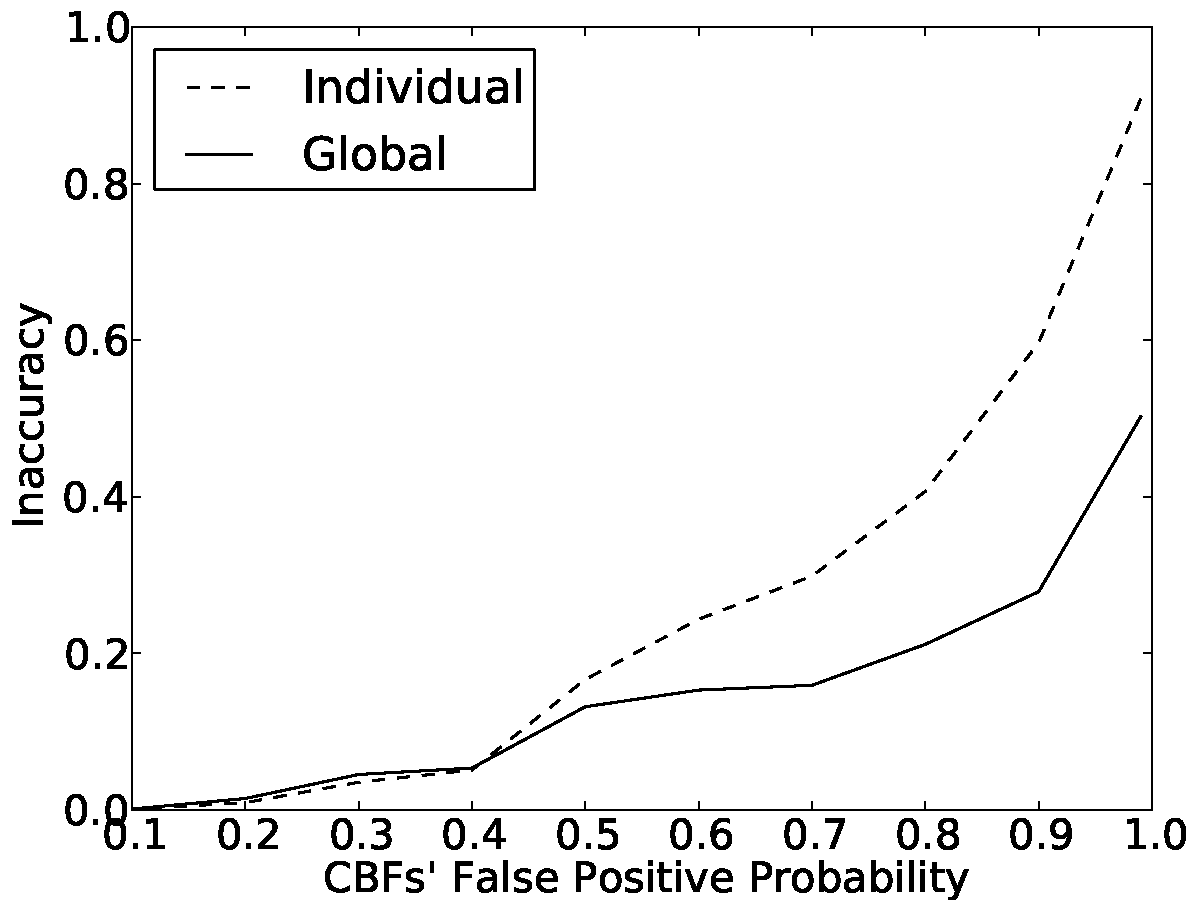
\includegraphics[width=0.33\linewidth]{images/s18x2805x11x4.pdf}
}\hspace*{-0.7em}
\subfigure[Synthetic-2805-50-16]{
 \label{fig:_2805_50_16}  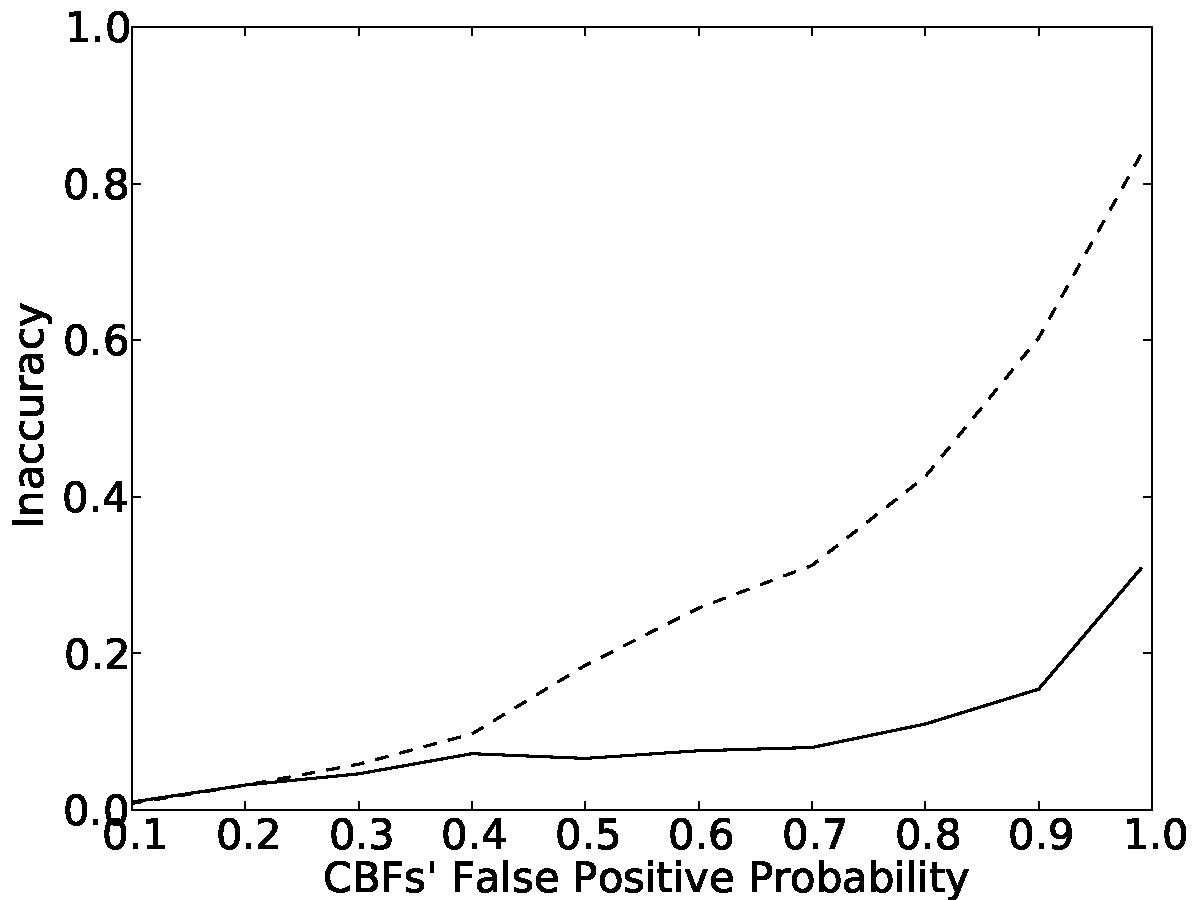
\includegraphics[width=0.33\linewidth]{images/s18x2805x50x16.pdf}
}\hspace*{-0.7em}
\subfigure[Synthetic-2805-100-30]{
\label{fig:s_2805_100_30}  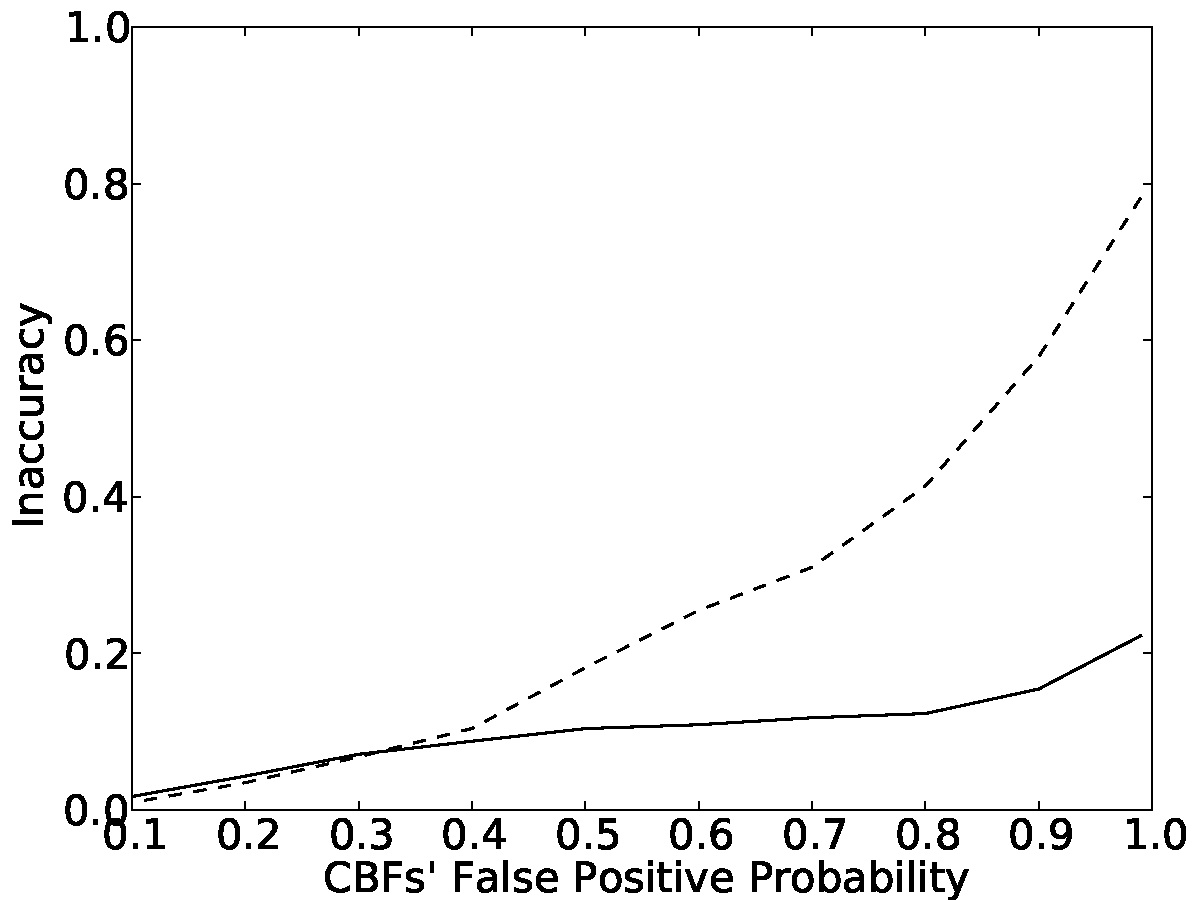
\includegraphics[width=0.33\linewidth]{images/s18x2805x100x30.pdf}
}
\caption{Synthetic data sets with increasing trace sizes}
\label{fig:perf_results_sim_trace_size}
\end{figure}

Keeping the same number of devices, while increasing the length of the
mobility traces also improves the Precedence Filter's global accuracy, as
depicted in Figure \ref{fig:perf_results_sim_trace_size}. For instance,
Figure \ref{fig:s_2805_100_30} shows that by increasing the average
and maximum values for mobility traces respectively to 30 and 100, our
technique offers a global error of about $15\%$, while providing $50\%$
of inaccuracy for individual information.

\begin{figure}[htb]
\subfigure[Synthetic-2805-11-4]{
\label{fig:s_2805_11_4}  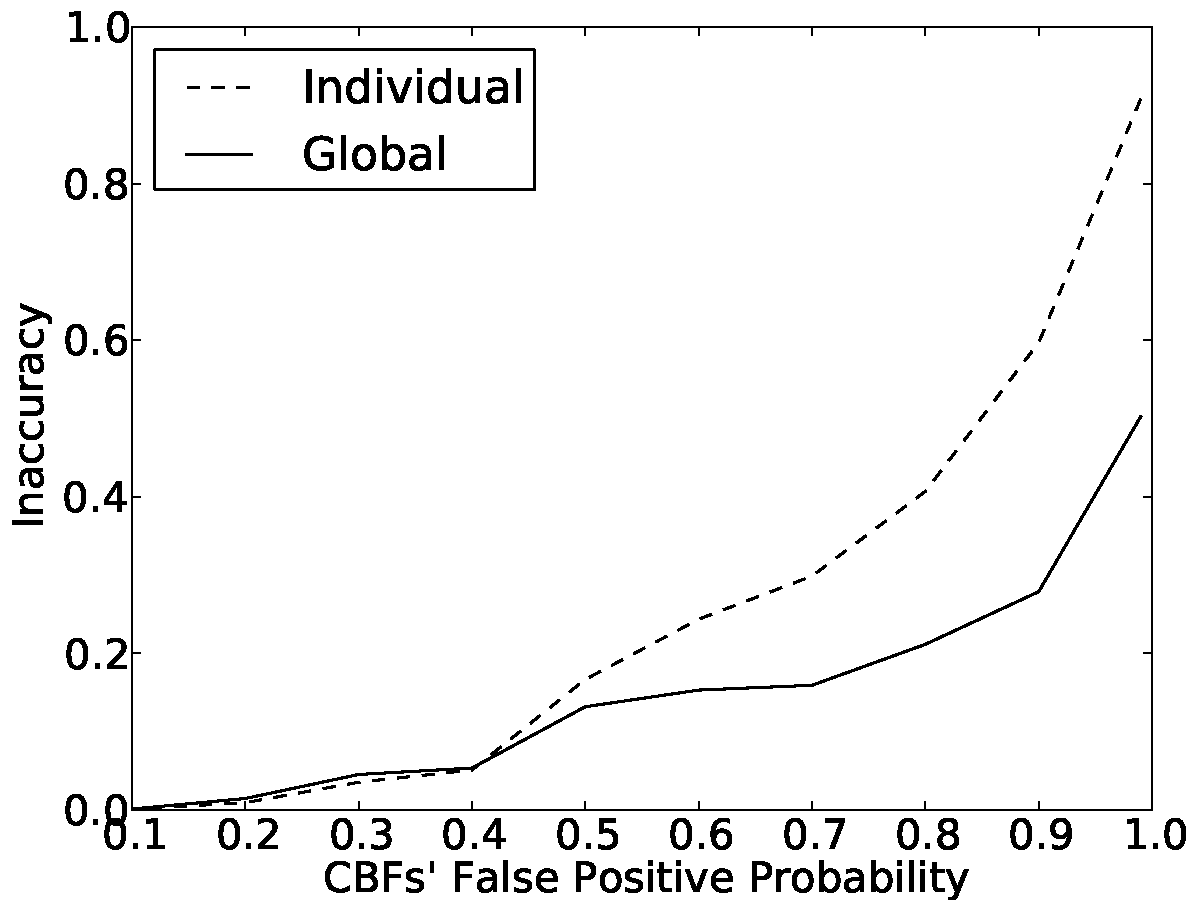
\includegraphics[width=0.33\linewidth]{images/s18x2805x11x4.pdf}
}\hspace*{-0.7em}
\subfigure[Synthetic-10000-50-16]{
 \label{fig:_2805_50_13}  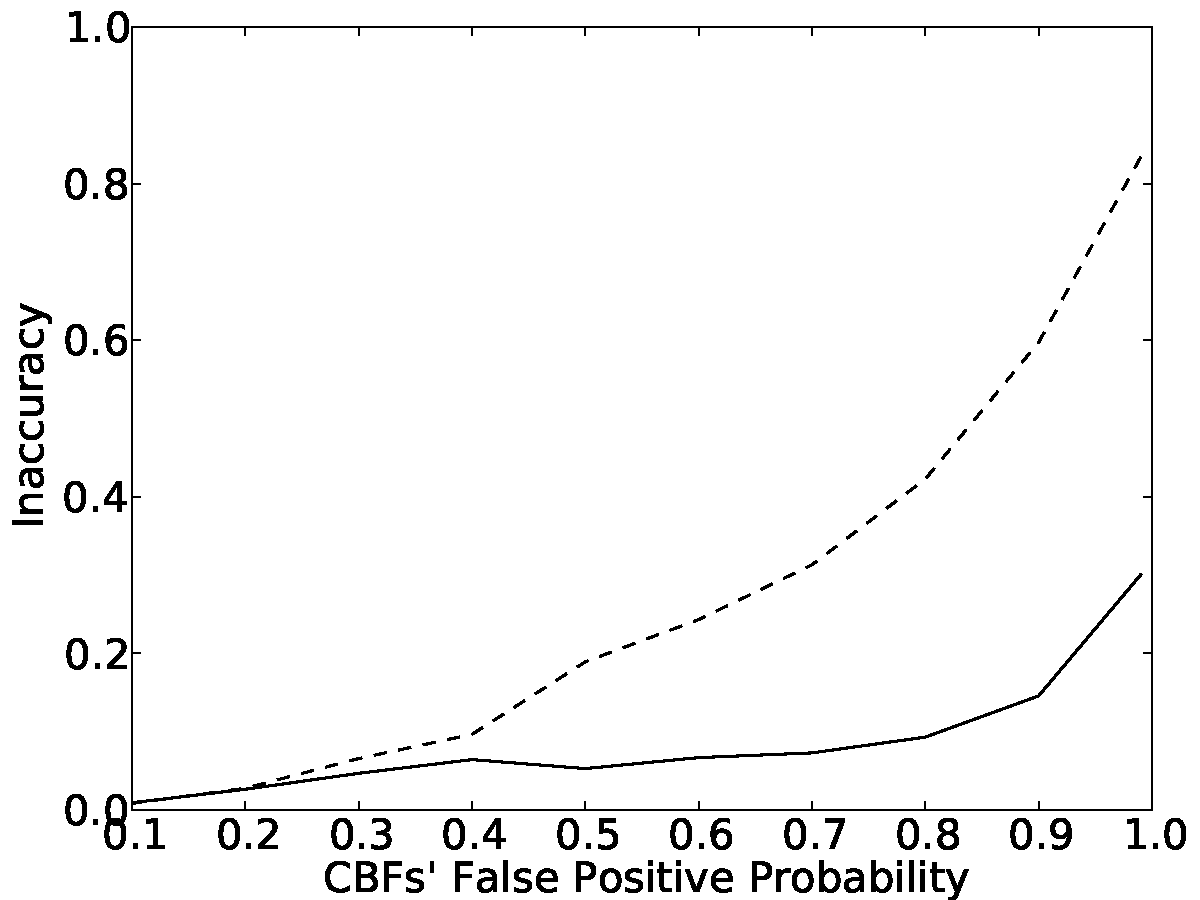
\includegraphics[width=0.33\linewidth]{images/s18x10000x50x16.pdf}
}\hspace*{-0.7em}
\subfigure[Synthetic-100000-100-30]{
 \label{fig:_2805_50_13}  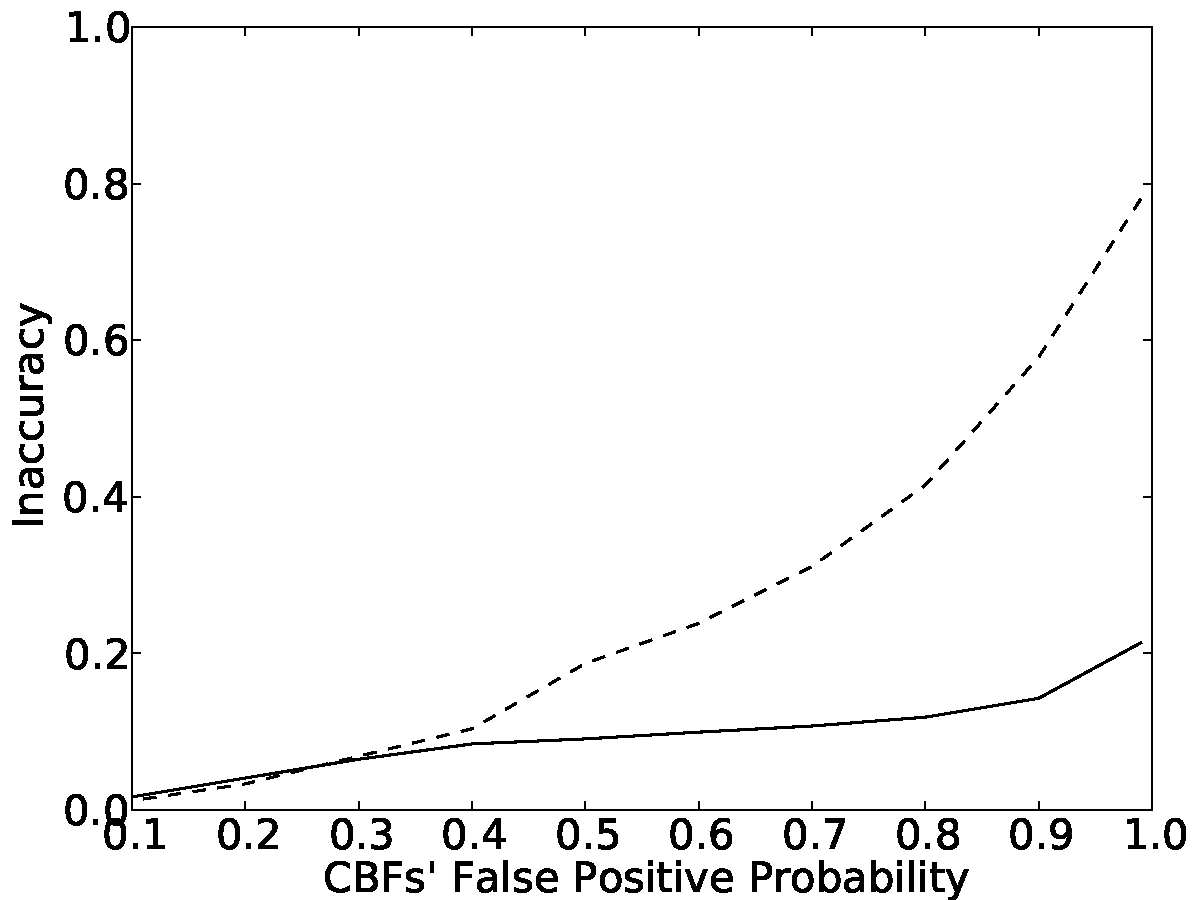
\includegraphics[width=0.33\linewidth]{images/s18x100000x100x30.pdf}
}
\caption{Synthetic data sets with increasing number of devices and
  trace sizes}
\label{fig:perf_results_sim_devices_traces}
\end{figure}

Increasing both the number of devices and the length of the mobility
traces yields the better results, which is not surprising given both
the previous results.

In a scenario with 100 000 users whose maximum and average mobility
trace sizes are respectively 100 and 30, depicted in Figure
b\ref{fig:_2805_50_13}, our technique has a global inaccuracy a little
higher than $10\%$ while providing an individual inaccuracy of $50\%$.
This means that, on average, half of the information about individual
transitions is wrong, which we consider to be a value compatible with
plausible deniability.  Recapitulating, our technique registers
information user transitions. Each user has a set of transitions, and
the individual metric measures, in average, the percentage of those
which are fictitious/false.  The global metric, on the other hand,
returns the average error regarding the information about the
popularity of specific transitions/paths. Increasing the false
positive probability of CBFs increases the total number of occurrences
of transitions, which is why the individual accuracy drops; yet the
relative weight of each transition (ratio) remains more stable, thus
the behavior of the global inaccuracy lines.

\section{Summary}
\label{sec:ct-summary}

Information about the flows of people at a macroscopic level can be used as
a decision support tool in several scenarios as it allows, to a
certain level, the understanding of people's behavior as a whole.  It
is therefore a very useful type of information.  However, to acquire
this type of macroscopic  information, one must collect individual
information (which in terms of privacy can be dangerous) about each
person. In light of these facts, we introduced and benchmarked an new
technique called \emph{Precedence Filters} which provides accurate
information at a macroscopic level without risking the individual
privacy of each user. It accomplishes this by ensuring that the
information regarding individuals can be plausibly denied.

Being based upon Vector Clocks and Counting Bloom Filters, this
technique is a compelling argument in proving that stochastic
summarizing techniques can be a viable building tool for privacy
preserving scenarios.


%%% Local Variables:
%%% mode: latex
%%% TeX-master: "../thesis"
%%% End:
